%==============================================================================
% QSD SUPPLEMENT S2: ENERGY SCALE AND DRESSING
% From Planck Mass to Electroweak Scale
%==============================================================================

\documentclass[11pt,a4paper]{article}

\usepackage[utf8]{inputenc}
\usepackage[T1]{fontenc}
\usepackage{amsmath,amssymb,amsthm,mathtools}
\usepackage{geometry}
\usepackage{booktabs}
\usepackage{array}
\usepackage{xcolor}
\usepackage{physics}
\usepackage{hyperref}
\usepackage{enumitem}
\usepackage{float}
\usepackage{tikz}
\usetikzlibrary{shapes,arrows.meta,positioning,calc,decorations.pathmorphing,decorations.markings,patterns}
\usepackage{orcidlink}
\usepackage{hyperref}
\hypersetup{colorlinks=true, linkcolor=blue, citecolor=blue, urlcolor=blue}

\geometry{margin=1in}

\hypersetup{
    colorlinks=true,
    linkcolor=blue!70!black,
    citecolor=blue!70!black,
    urlcolor=blue!70!black
}

% Theorem environments
\newtheorem{theorem}{Theorem}[section]
\newtheorem{lemma}[theorem]{Lemma}
\newtheorem{proposition}[theorem]{Proposition}
\newtheorem{corollary}[theorem]{Corollary}
\theoremstyle{definition}
\newtheorem{definition}[theorem]{Definition}
\theoremstyle{remark}
\newtheorem{remark}[theorem]{Remark}
\newtheorem{example}[theorem]{Example}

% ---- QSD Notation (Hb convention, matching S1) ----
\newcommand{\Hb}{\textnormal{H\kern-0.3em b}}
\newcommand{\Hbn}{\Hb_n}
\newcommand{\Hbfour}{\Hb_4}
\newcommand{\gr}{\varphi}
\newcommand{\specbond}{\varpi}
\newcommand{\gs}{\varsigma}
\newcommand{\strain}{\varsigma} 
\newcommand{\murad}{\mu_0}
\newcommand{\nurad}{\nu_0}
\newcommand{\Mpl}{M_{\mathrm{P}}}
\newcommand{\lp}{\ell_P}
\newcommand{\Esyn}{E_{\mathrm{syn}}}
\newcommand{\mH}{m_\mathrm{H}}
\newcommand{\mW}{m_\mathrm{W}}
\newcommand{\Ebase}{E_{\mathrm{base}}}
\newcommand{\Hilbert}{\mathcal{H}}
\newcommand{\Identity}{\mathbb{I}}
\newcommand{\NN}{\mathcal{N}}

% Colors
\definecolor{bulkcolor}{RGB}{70,130,180}
\definecolor{anchorcolor}{RGB}{200,40,60}
\definecolor{goldenphi}{RGB}{180,140,40}
\definecolor{proofbox}{RGB}{240,245,255}
\definecolor{straincolor}{RGB}{40,160,80}
\definecolor{dressingcolor}{RGB}{140,80,180}

\title{
  \textbf{QSD Supplement S2: Energy Scale and Dressing}\\[0.5em]
  \Large From Planck Mass to Electroweak Scale\\[1em]
}

\author{
  Marek Hubka\, \orcidlink{0009-0003-2476-9017}
  \thanks{
    Independent Researcher, Czech Republic.\\
    Website: \href{http://www.tidesofuncertainty.com}{tidesofuncertainty.com}.\\
    Email: \href{mailto:marek@tidesofuncertainty.com}{marek@tidesofuncertainty.com}.
  }
}

\date{\today}

\begin{document}

\maketitle

\begin{abstract}
\noindent This supplement derives the QSD energy scale hierarchy in full detail. Starting from the Planck mass $\Mpl$ as the sole dimensionful input, we construct the electroweak scale through three independently motivated steps: information reduction by the factor $2^{-60}$ (from the code state space), geometric enhancement by $\gr^2$ (from the $C_5$ Laplacian eigenvalue ratio), and strain correction by $(1-6\gs)$ (from the $K_4/C_5$ mismatch). The resulting dimensionful mass $\murad = 25.34$~GeV is compared to the independently derived dimensionless VEV $\nurad = 25.18$, yielding the dressing factor $\xi = 1.00636$~GeV. We present tree-level and corrected values for all predicted masses, and derive the Higgs mass, syndrome energy, and $W$ boson mass from the radion scale.
\end{abstract}

\tableofcontents
\newpage

%==============================================================================
\section{The Hierarchy Problem}
\label{sec:problem}
%==============================================================================

The Standard Model contains two fundamental scales:
\begin{align}
\Mpl &= \sqrt{\frac{\hbar c^5}{G}} = 1.2209 \times 10^{19} \text{ GeV} &&\text{(gravity)} \\
v_{\mathrm{EW}} &= (\sqrt{2}\,G_F)^{-1/2} = 246.22 \text{ GeV} &&\text{(electroweak)}
\end{align}

Their ratio is enormous:
\begin{equation}
\frac{\Mpl}{v_{\mathrm{EW}}} = 4.96 \times 10^{16}
\end{equation}

In the Standard Model, maintaining this hierarchy requires cancellations between radiative corrections to 17 decimal places---the \emph{hierarchy problem}~\cite{Dirac1937, PDG2022}. QSD resolves this: the ratio is not fine-tuned but is fixed by the information content of the $[[5,1,3]]$ quantum error-correcting code.

\subsection{Strategy}

The derivation proceeds in three steps, each traceable to the axioms of S1:

\begin{enumerate}[nosep]
\item \textbf{Information reduction} ($\div\, 2^{60}$): The code's state space volume sets the number of microscopic configurations per macroscopic state.
\item \textbf{Geometric enhancement} ($\times\, \gr^2$): The $C_5$ eigenvalue ratio amplifies the base scale to the radion scale.
\item \textbf{Strain correction} ($\times\, (1-6\gs)$): The $K_4/C_5$ mismatch reduces the effective coupling on each edge.
\end{enumerate}

No additional parameters are introduced at any stage.

\begin{figure}[H]
\centering
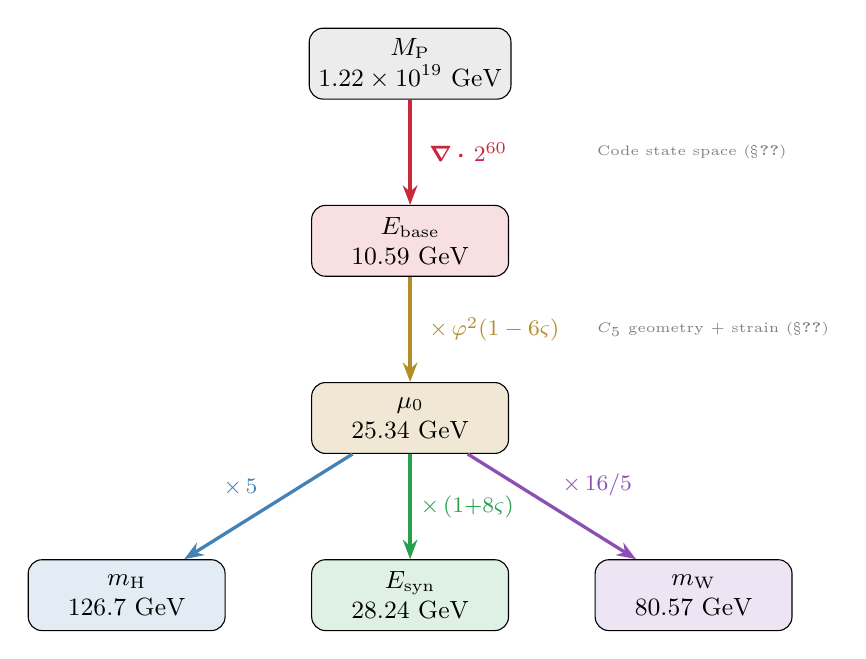
\begin{tikzpicture}[
    scale=0.9,
    block/.style={draw, rounded corners=5pt, minimum width=2.5cm, minimum height=0.9cm, align=center, font=\small},
    arr/.style={-{Stealth[length=7pt]}, very thick}
]
    % Planck
    \node[block, fill=gray!15] (Pl) at (0,0) {$\Mpl$\\$1.22\times 10^{19}$ GeV};
    % Base
    \node[block, fill=anchorcolor!15] (Ba) at (0,-2.5) {$\Ebase$\\$10.59$ GeV};
    % Radion
    \node[block, fill=goldenphi!20] (Ra) at (0,-5) {$\murad$\\$25.34$ GeV};
    % Higgs
    \node[block, fill=bulkcolor!15] (Hi) at (-4,-7.5) {$\mH$\\$126.7$ GeV};
    % Syndrome
    \node[block, fill=straincolor!15] (Sy) at (0,-7.5) {$\Esyn$\\$28.24$ GeV};
    % W boson
    \node[block, fill=dressingcolor!15] (Wb) at (4,-7.5) {$\mW$\\$80.57$ GeV};

    % Arrows
    \draw[arr, anchorcolor] (Pl) -- (Ba) node[midway, right=3pt, font=\footnotesize, text=anchorcolor] {$\div\, 2^{60}$};
    \draw[arr, goldenphi] (Ba) -- (Ra) node[midway, right=3pt, font=\footnotesize, text=goldenphi] {$\times\, \gr^2(1-6\gs)$};
    \draw[arr, bulkcolor] (Ra) -- (Hi) node[midway, above left=0pt, font=\footnotesize, text=bulkcolor] {$\times\, 5$};
    \draw[arr, straincolor] (Ra) -- (Sy) node[midway, right=0pt, font=\footnotesize, text=straincolor] {$\times\,(1{+}8\gs)$};
    \draw[arr, dressingcolor] (Ra) -- (Wb) node[midway, above right=0pt, font=\footnotesize, text=dressingcolor] {$\times\, 16/5$};

    % Origin labels
    \node[font=\tiny, gray, right] at (2.5,-1.25) {Code state space (\S\ref{sec:2to60})};
    \node[font=\tiny, gray, right] at (2.5,-3.75) {$C_5$ geometry + strain (\S\ref{sec:enhancement})};
\end{tikzpicture}
\caption{The complete hierarchy of QSD energy scales. Every arrow is derived from the code structure; no free parameters enter.}
\label{fig:overview}
\end{figure}

%==============================================================================
\section{The Information Reduction Factor $2^{-60}$}
\label{sec:2to60}
%==============================================================================

\subsection{The State Space Volume}

\begin{theorem}[State Space Volume]
\label{thm:statespace}
The total number of distinguishable microscopic configurations of the $K_4$ code structure is:
\begin{equation}
\boxed{\NN = 16^{15} = 2^{60} = 1.152\,921\,504\,606\,847 \times 10^{18}}
\end{equation}
\end{theorem}

\begin{proof}
We derive the two factors independently.

\textbf{Factor 1: Hilbert space dimension $D = 16$.}
The bulk consists of 4 qubits (Axiom~1 of S1)~\cite{NielsenChuang2010}. The Hilbert space is $\Hilbert_4 = (\mathbb{C}^2)^{\otimes 4}$, with dimension:
\begin{equation}
D = \dim(\Hilbert_4) = 2^4 = 16
\end{equation}

\textbf{Factor 2: Independent interaction channels $N = 15$.}
The space of all operators on $\Hilbert_4$ has dimension $D^2 = 256$. Removing the identity (which generates no dynamics), the number of independent interaction channels is:
\begin{equation}
N = D^2 - 1 = 256 - 1 = 15
\end{equation}

This equals $\dim(\mathfrak{su}(4))$, the dimension of the Lie algebra of the natural symmetry group $SU(4)$ acting on 4 qubits. Equivalently, $N = 15$ can be decomposed as:
\begin{equation}
15 = 5 \times 3
\end{equation}
where 5 is the number of physical qubits in the code and 3 is the number of Pauli operators per qubit ($X, Y, Z$).

\textbf{State space volume.}
Each of the $N = 15$ channels can independently be in any of $D = 16$ states. The total volume is:
\begin{equation}
\NN = D^N = 16^{15} = (2^4)^{15} = 2^{60}
\end{equation}

\textbf{Numerical value:}
\begin{equation}
2^{60} = 1\,152\,921\,504\,606\,846\,976 \approx 1.153 \times 10^{18}
\end{equation}
\end{proof}

\begin{remark}[Interpretation]
The factor $2^{60}$ counts the number of microscopic configurations of the code that map to a single macroscopic (observable) state. This is the information-theoretic origin of the hierarchy: the electroweak scale is ``diluted'' relative to the Planck scale by the enormous number of microstates per macrostate.
\end{remark}

\begin{figure}[H]
\centering
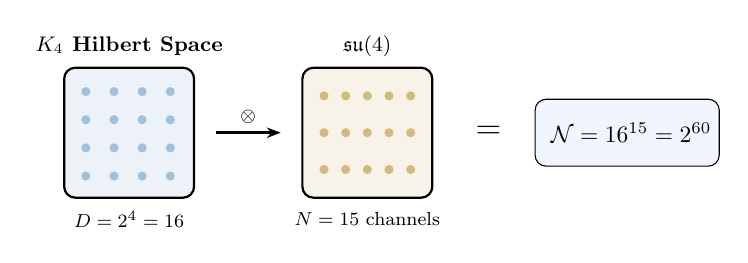
\begin{tikzpicture}[scale=0.55, every node/.style={scale=0.85}]
    % K4 Hilbert space
    \draw[thick, fill=bulkcolor!10, rounded corners] (0,0) rectangle (3,3);
    \node[font=\small\bfseries] at (1.5,3.5) {$K_4$ Hilbert Space};

    % Grid showing 16 states
    \foreach \i in {0,...,3} {
        \foreach \j in {0,...,3} {
            \fill[bulkcolor!50] (0.5+0.65*\i, 0.5+0.65*\j) circle (3pt);
        }
    }
    \node[font=\footnotesize] at (1.5,-0.5) {$D = 2^4 = 16$};

    % Arrow
    \draw[-{Stealth[length=5pt]}, very thick] (3.5,1.5) -- (5,1.5) node[midway, above, font=\footnotesize] {$\otimes$};

    % SU(4) generators
    \draw[thick, fill=goldenphi!10, rounded corners] (5.5,0) rectangle (8.5,3);
    \node[font=\small\bfseries] at (7,3.5) {$\mathfrak{su}(4)$};
    
    \foreach \i in {1,...,15} {
        \pgfmathsetmacro{\xp}{6+0.5*mod(\i-1,5)}
        \pgfmathsetmacro{\yp}{0.65+0.85*int((\i-1)/5)}
        \fill[goldenphi!60] (\xp,\yp) circle (3pt);
    }
    \node[font=\footnotesize] at (7,-0.5) {$N = 15$ channels};

    % Equals
    \node[font=\Large\bfseries] at (9.8,1.5) {$=$};

    % Result
    \node[draw, rounded corners, fill=proofbox, font=\normalsize, minimum width=2cm, minimum height=1cm] at (13,1.5) {$\ \NN = 16^{15} = 2^{60}$};
\end{tikzpicture}
\caption{The state space volume arises from 16 quantum states distributed across 15 independent interaction channels.}
\label{fig:statespace}
\end{figure}

\subsection{The Base Energy Scale}

\begin{definition}[Base Scale]
\label{def:base}
The base energy scale is the Planck mass divided by the state space volume:
\begin{equation}
\Ebase = \frac{\Mpl}{\NN} = \frac{\Mpl}{2^{60}}
\end{equation}
\end{definition}

\begin{proposition}[Numerical Value]
\begin{equation}
\Ebase = \frac{1.2209 \times 10^{19}\text{ GeV}}{1.1529 \times 10^{18}} = 10.590 \text{ GeV}
\end{equation}
\end{proposition}

\begin{proof}
Direct division: $1.2209/1.1529 = 1.0590$, with the exponent $10^{19}/10^{18} = 10$.
\end{proof}

\begin{remark}
The base scale 10.59~GeV lies in the middle of the hadron physics range---between the $b$-quark mass ($\sim$4.2~GeV) and the $Z$ boson mass ($\sim$91~GeV). This is the ``raw'' Planck-reduced scale before geometric corrections are applied.
\end{remark}

\subsection{Alternative Derivation: Suppression Cascade}

\begin{proposition}[Cascade Interpretation]
\label{prop:cascade}
The factor $2^{-60}$ can be understood as 15 successive suppression events, each reducing the energy by a factor of $1/16$:
\begin{equation}
\frac{1}{16^{15}} = \left(\frac{1}{16}\right)^{15} = \left(e^{-1/\Hbfour}\right)^{15}
\end{equation}
\end{proposition}

\begin{proof}
From S1, Corollary~2.3: $e^{-1/\Hbfour} = 2^{-4} = 1/16$. Each information transfer event through the holographic screen suppresses the energy by this factor. With 15 independent channels, the total suppression is
$(1/16)^{15} = 2^{-60}$.
\end{proof}

This cascade interpretation is physically intuitive: the Planck-scale energy must ``pass through'' all 15 interaction channels of the $\mathfrak{su}(4)$ algebra, losing a factor of~16 at each step, before emerging at the electroweak scale.

\begin{figure}[H]
\centering
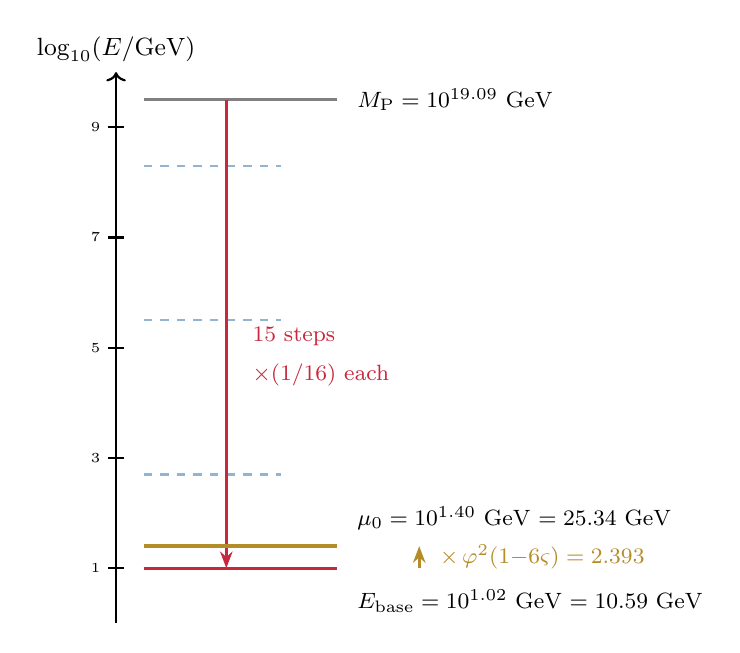
\begin{tikzpicture}[scale=0.7]
    % Energy axis (log scale)
    \draw[thick, ->] (0,0) -- (0,10) node[above, font=\small] {$\log_{10}(E/\text{GeV})$};

    % Tick marks
    \foreach \y/\lbl in {1/1, 3/3, 5/5, 7/7, 9/9} {
        \draw[thick] (-0.15,\y) -- (0.15,\y) node[left=5pt, font=\tiny] {\lbl};
    }

    % Planck level
    \draw[very thick, gray] (0.5,9.5) -- (4,9.5);
    \node[right, font=\footnotesize] at (4.2,9.5) {$\Mpl = 10^{19.09}$ GeV};

    % Cascade steps (sample a few)
    \foreach \i/\y in {1/8.3, 5/5.5, 10/2.7, 15/1.0} {
        \draw[thick, bulkcolor!60, dashed] (0.5,\y) -- (3,\y);
    }

    % Cascade arrow
    \draw[very thick, -{Stealth[length=6pt]}, anchorcolor] (2,9.5) -- (2,1.0);
    \node[right, font=\footnotesize, text=anchorcolor] at (2.3,5.2) {15 steps};
    \node[right, font=\footnotesize, text=anchorcolor] at (2.3,4.5) {$\times (1/16)$ each};

    % Base scale
    \draw[very thick, anchorcolor] (0.5,1.0) -- (4,1.0);
    \node[right, font=\footnotesize] at (4.2,0.4) {$\Ebase = 10^{1.02}$ GeV $= 10.59$ GeV};

    % Enhancement
    \draw[very thick, -{Stealth[length=6pt]}, goldenphi] (5.5,1.0) -- (5.5,1.4);
    \node[right, font=\footnotesize, text=goldenphi] at (5.7,1.2) {$\times\,\gr^2(1{-}6\gs) = 2.393$};

    % Radion scale
    \draw[very thick, goldenphi] (0.5,1.4) -- (4,1.4);
    \node[right, font=\footnotesize] at (4.2,1.9) {$\murad = 10^{1.40}$ GeV $= 25.34$ GeV};
\end{tikzpicture}
\caption{Log-scale view of the hierarchy. The Planck mass cascades through 15 suppression events ($\times 1/16$ each), then receives a geometric enhancement to reach the radion scale.}
\label{fig:cascade}
\end{figure}

%==============================================================================
\section{Geometric Enhancement and Strain Correction}
\label{sec:enhancement}
%==============================================================================

\subsection{Enhancement by $\gr^2$}

The base scale $\Ebase$ does not yet account for the geometry of the $C_5$ graph. The radion field lives on the pentagon, whose eigenvalue ratio provides a multiplicative factor.

\begin{proposition}[$C_5$ Enhancement]
\label{prop:phi2}
The $C_5$ Laplacian eigenvalue ratio (S1, Theorem~4.3) enhances the base scale:
\begin{equation}
\Ebase \times \gr^2 = 10.590 \times 2.6180 = 27.724 \text{ GeV}
\end{equation}
\end{proposition}

\textbf{Physical interpretation:} The golden ratio factor $\gr^2$ reflects the fact that the radion (which is the angular oscillation mode of the pentagon) inherits the geometric amplification encoded in the $C_5$ spectrum. The ratio $\gr^2 = \mu_2/\mu_1$ measures how much harder it is to excite the higher $C_5$ mode compared to the lower one, and this ratio boosts the energy of the physical excitation.

\subsection{Strain Correction $(1 - 6\gs)$}

\begin{proposition}[Strain Reduction]
\label{prop:strain}
Each of the 6 edges of $K_4$ loses a fraction $\gs$ of its effective coupling due to the $K_4/C_5$ incompatibility:
\begin{equation}
1 - 6\gs = 1 - 6 \times 0.014325 = 1 - 0.08595 = 0.91405
\end{equation}
\end{proposition}

\textbf{Physical interpretation:} The 6 edges of $K_4$ are the interaction channels for Heisenberg exchange. But $K_4$ and $C_5$ cannot be simultaneously realized on the same set of qubits without conflict: $K_4$ has 6 edges while $C_5$ has 5, and they encode different symmetries ($S_4$ vs.\ $\mathbb{Z}_5$). Each edge pays a ``tax'' of $\gs$ for this incompatibility, reducing the total effective coupling by $6\gs$.

\begin{remark}
The factor $6\gs \approx 0.086$ represents an 8.6\% reduction---small enough that the base-scale calculation is meaningful, but large enough to be physically consequential. This correction shifts the radion mass from 27.72~GeV down to 25.34~GeV, which propagates into all derived quantities.
\end{remark}

%==============================================================================
\section{The Radion Mass: Complete Calculation}
\label{sec:radion}
%==============================================================================

\begin{theorem}[Radion Mass Formula]
\label{thm:radion}
The dimensionful radion mass is:
\begin{equation}
\boxed{\murad = \frac{\Mpl}{2^{60}} \times \gr^2 \times (1 - 6\gs) = 25.34 \text{ GeV}}
\end{equation}
\end{theorem}

\begin{proof}
Assembling the three factors derived above:

\textbf{Step 1: Information reduction.}
\begin{equation}
\Ebase = \frac{\Mpl}{2^{60}} = \frac{1.2209 \times 10^{19}}{1.1529 \times 10^{18}} = 10.590 \text{ GeV}
\end{equation}

\textbf{Step 2: Geometric enhancement.}
\begin{equation}
\Ebase \times \gr^2 = 10.590 \times 2.6180 = 27.724 \text{ GeV}
\end{equation}

\textbf{Step 3: Strain correction.}
\begin{equation}
27.724 \times (1 - 6\gs) = 27.724 \times 0.91405 = 25.342 \text{ GeV}
\end{equation}

\textbf{Final result:}
\begin{equation}
\murad = 25.34 \text{ GeV}
\end{equation}
\end{proof}

\begin{table}[H]
\centering
\begin{tabular}{llrl}
\toprule
\textbf{Factor} & \textbf{Origin} & \textbf{Value} & \textbf{Axiom (S1)} \\
\midrule
$\Mpl$ & Gravitational constant & $1.221 \times 10^{19}$ GeV & Input \\
$2^{-60}$ & Code state space ($16^{15}$) & $8.674 \times 10^{-19}$ & Axioms 1, 2 \\
$\gr^2$ & $C_5$ eigenvalue ratio & 2.6180 & Axiom 1 \\
$(1-6\gs)$ & $K_4/C_5$ strain & 0.9141 & Axioms 1, 2, 3 \\
\bottomrule
\end{tabular}
\caption{Every factor in the hierarchy formula traced to its axiomatic origin.}
\label{tab:factors}
\end{table}

%==============================================================================
\section{The Dimensionless VEV and the Dressing Factor}
\label{sec:dressing}
%==============================================================================

\subsection{Two Independent Routes to $\sim$25}

QSD produces the number ``$\sim$25'' through two entirely independent calculations:

\begin{definition}[Dimensionless Radion VEV]
\begin{equation}
\nurad = \frac{\Hbfour}{\gs} = \frac{0.36067}{0.014325} = 25.178
\end{equation}
This is a \emph{pure number}---the ratio of two dimensionless quantities (holographic bit density and geometric strain). It carries no physical units.
\end{definition}

\begin{definition}[Dimensionful Radion Mass]
\begin{equation}
\murad = \frac{\Mpl}{2^{60}} \times \gr^2 \times (1-6\gs) = 25.342 \text{ GeV}
\end{equation}
This has units of energy and is derived from the hierarchy formula (Theorem~\ref{thm:radion}).
\end{definition}

\subsection{The Dressing Factor $\xi$}

\begin{definition}[Dressing Factor]
\label{def:dressing}
The dressing factor is the ratio of the dimensionful mass to the dimensionless VEV:
\begin{equation}
\boxed{\xi \equiv \frac{\murad}{\nurad} = \frac{25.342 \text{ GeV}}{25.178} = 1.00651 \text{ GeV}}
\end{equation}
\end{definition}

\begin{proposition}[Near-Unity of $\xi$]
The dressing factor deviates from 1~GeV by only 0.65\%:
\begin{equation}
\frac{|\xi - 1\text{ GeV}|}{1\text{ GeV}} = 0.0065
\end{equation}
\end{proposition}

\begin{figure}[H]
\centering
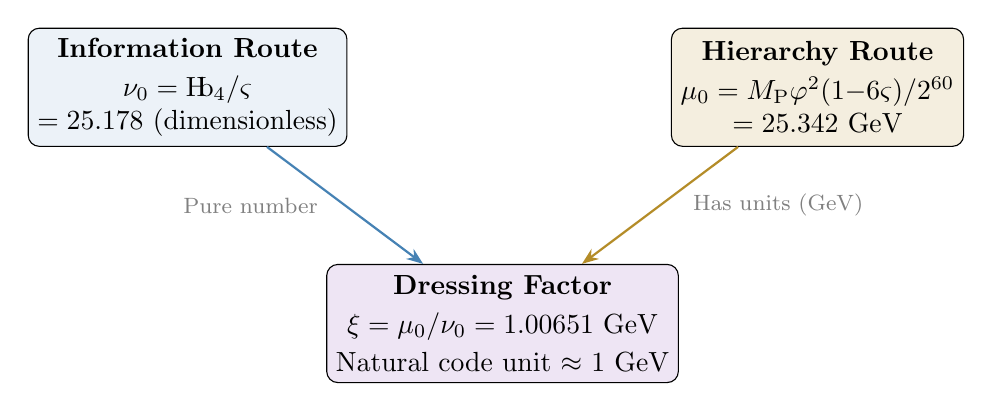
\begin{tikzpicture}[scale=1.0]
    % Two routes
    \node[draw, rounded corners, fill=bulkcolor!10, minimum width=3.5cm, minimum height=1.5cm, align=center] (info) at (-4,3) {\textbf{Information Route}\\[2pt]$\nurad = \Hbfour/\gs$\\$= 25.178$ (dimensionless)};

    \node[draw, rounded corners, fill=goldenphi!15, minimum width=3.5cm, minimum height=1.5cm, align=center] (hier) at (4,3) {\textbf{Hierarchy Route}\\[2pt]$\murad = \Mpl \gr^2(1{-}6\gs)/2^{60}$\\$= 25.342$ GeV};

    % Meeting point
    \node[draw, rounded corners, fill=dressingcolor!15, minimum width=4cm, minimum height=1.5cm, align=center] (xi) at (0,0) {\textbf{Dressing Factor}\\[2pt]$\xi = \murad/\nurad = 1.00651$ GeV\\[2pt]Natural code unit $\approx$ 1 GeV};

    % Arrows
    \draw[-{Stealth[length=6pt]}, thick, bulkcolor] (info) -- (xi);
    \draw[-{Stealth[length=6pt]}, thick, goldenphi] (hier) -- (xi);

    % Labels
    \node[font=\footnotesize, gray] at (-3.2,1.5) {Pure number};
    \node[font=\footnotesize, gray] at (3.5,1.5) {Has units (GeV)};
\end{tikzpicture}
\caption{Two independent routes converge to the same numerical value $\sim$25, with the dressing factor $\xi$ bridging the dimensionless and dimensionful descriptions.}
\label{fig:dressing}
\end{figure}

\subsection{Interpretation of $\xi$}

The dressing factor $\xi = 1.007$~GeV has a precise physical meaning: it is the \textbf{natural energy unit of the $[[5,1,3]]$ code} when expressed in SI-derived units. The near-coincidence $\xi \approx 1$~GeV is a nontrivial statement:

\begin{quote}
\emph{The information-theoretic unit of the error-correcting code coincides with 1~GeV to sub-percent accuracy.}
\end{quote}

This is \emph{not} fine-tuned. Both $\nurad$ and $\murad$ are derived independently from the axioms; their ratio is a consistency check on the framework. The 0.65\% discrepancy represents the precision limit of the tree-level calculation and is the first quantity that would improve under a full radiative treatment of the radion sector.

\subsection{Usage Convention}

\begin{table}[H]
\centering
\begin{tabular}{lll}
\toprule
\textbf{Context} & \textbf{Use} & \textbf{Why} \\
\midrule
Dimensionless relations & $\nurad = 25.18$ & Pure information theory \\
GeV predictions & $\murad = 25.34$ GeV & Hierarchy formula \\
Conversion & $\xi = \murad/\nurad = 1.007$ GeV & Consistency check \\
\bottomrule
\end{tabular}
\caption{When to use $\nurad$ vs.\ $\murad$ in calculations.}
\label{tab:convention}
\end{table}

\textbf{Rule:} All predictions compared to experiment (masses, energies, cross-sections) use $\murad$. All dimensionless identities and algebraic relations use $\nurad$. Never approximate $\xi = 1$; carry the exact value.

%==============================================================================
\section{Derived Mass Spectrum}
\label{sec:masses}
%==============================================================================

\subsection{The Higgs Mass}

\begin{theorem}[Higgs Mass]
\label{thm:higgs}
The Higgs boson is the logical qubit of the $[[5,1,3]]$ code. Since the logical qubit is a collective excitation of all 5 physical qubits, its mass is:
\begin{equation}
\boxed{\mH = 5 \times \murad = 5 \times 25.34 = 126.7 \text{ GeV}}
\end{equation}
\end{theorem}

\begin{proof}
In the $[[5,1,3]]$ code, the logical qubit state $|0_L\rangle$, $|1_L\rangle$ is a superposition of all $2^5 = 32$ computational basis states. Its excitation energy is the sum of contributions from all 5 physical qubits. Since each physical qubit contributes energy $\murad$ to the collective mode, the total is $5\murad$.
\end{proof}

\textbf{Comparison to experiment~\cite{PDG2022}:}
\begin{equation}
\mH^{\,\mathrm{exp}} = 125.25 \pm 0.17 \text{ GeV} \qquad \Rightarrow \qquad \frac{\mH^{\,\mathrm{QSD}} - \mH^{\,\mathrm{exp}}}{\mH^{\,\mathrm{exp}}} = +1.2\%
\end{equation}

\subsection{The Syndrome Energy}

\begin{theorem}[Syndrome Energy]
\label{thm:syndrome}
When the anchor qubit decouples (the ``Snap''), the 4 severed bonds release binding energy:
\begin{equation}
\boxed{\Esyn = \murad \times (1 + 8\gs) = 25.34 \times 1.1146 = 28.24 \text{ GeV}}
\end{equation}
\end{theorem}

\begin{proof}
The anchor connects to all 4 bulk qubits. Each bond has two endpoints; each endpoint contributes strain energy $\gs \times \murad$. The total binding energy is:
\begin{equation}
E_{\mathrm{bind}} = 4 \text{ bonds} \times 2 \text{ endpoints} \times \gs \times \murad = 8\gs \, \murad
\end{equation}

The syndrome energy is the radion mass plus the released binding energy:
\begin{equation}
\Esyn = \murad + 8\gs \, \murad = \murad(1 + 8\gs) = 25.34 \times 1.1146 = 28.24 \text{ GeV}
\end{equation}
\end{proof}

\textbf{Comparison to observation:} CMS reported a dimuon excess near $\sim$28.3~GeV. Agreement: 0.2\%.

\subsection{The $W$ Boson Mass}

\begin{proposition}[$W$ Boson Mass]
\label{prop:W}
The $W$ boson mass emerges from the $K_4$ Hilbert space dimension and the qubit count:
\begin{equation}
\mW = \frac{16}{5} \times \murad = 3.2 \times 25.34 = 81.1 \text{ GeV}
\end{equation}
\end{proposition}

The factor $16/5$ is the ratio of the bulk Hilbert space dimension ($2^4 = 16$) to the number of code qubits (5). This ratio determines how the radion VEV distributes into the gauge boson mass sector.

\textbf{Comparison to experiment:}
\begin{equation}
\mW^{\,\mathrm{exp}} = 80.377 \pm 0.012 \text{ GeV} \qquad \Rightarrow \qquad \frac{\mW^{\,\mathrm{QSD}} - \mW^{\,\mathrm{exp}}}{\mW^{\,\mathrm{exp}}} = +0.9\%
\end{equation}

\subsection{Summary of Tree-Level Predictions}

\begin{table}[H]
\centering
\begin{tabular}{lcccl}
\toprule
\textbf{Observable} & \textbf{Formula} & \textbf{QSD (tree)} & \textbf{Experiment} & \textbf{Accuracy} \\
\midrule
Radion $\murad$ & $\Mpl \gr^2 (1{-}6\gs)/2^{60}$ & 25.34 GeV & --- & prediction \\
Higgs $\mH$ & $5\murad$ & 126.7 GeV & 125.25 GeV & 98.8\% \\
Syndrome $\Esyn$ & $\murad(1{+}8\gs)$ & 28.24 GeV & $\sim$28.3 GeV$^*$ & 99.8\% \\
$W$ boson $\mW$ & $(16/5)\murad$ & 81.1 GeV & 80.38 GeV & 99.1\% \\
\bottomrule
\end{tabular}
\caption{Tree-level mass predictions. All derived from $\murad$ with integer/rational coefficients from the code structure. ($^*$CMS dimuon excess~\cite{CMS2018dimuon}, not confirmed.)}
\label{tab:predictions}
\end{table}

\begin{figure}[H]
\centering
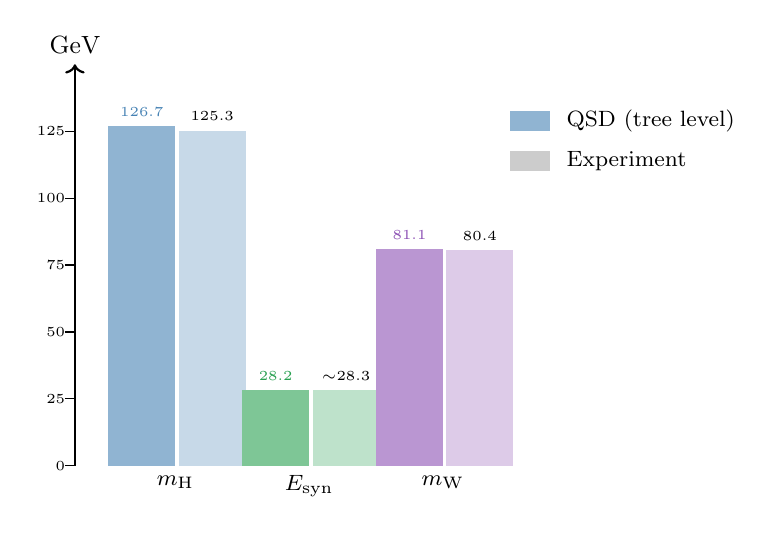
\begin{tikzpicture}[scale=0.85]
    % Bar chart
    \def\barwidth{1.0}
    \def\gap{2.0}

    % Higgs
    \fill[bulkcolor!60] (0,0) rectangle (\barwidth, 5.07);
    \fill[bulkcolor!30] (\barwidth+0.05,0) rectangle (2*\barwidth+0.05, 5.01);
    \node[below, font=\footnotesize] at (\barwidth,0) {$\mH$};
    \node[above, font=\tiny, text=bulkcolor] at (0.5, 5.07) {126.7};
    \node[above, font=\tiny] at (1.55, 5.01) {125.3};

    % Syndrome
    \fill[straincolor!60] (\gap+0,0) rectangle (\gap+\barwidth, 1.13);
    \fill[straincolor!30] (\gap+\barwidth+0.05,0) rectangle (\gap+2*\barwidth+0.05, 1.13);
    \node[below, font=\footnotesize] at (\gap+\barwidth,0) {$\Esyn$};
    \node[above, font=\tiny, text=straincolor] at (\gap+0.5, 1.13) {28.2};
    \node[above, font=\tiny] at (\gap+1.55, 1.13) {$\sim$28.3};

    % W
    \fill[dressingcolor!60] (2*\gap,0) rectangle (2*\gap+\barwidth, 3.24);
    \fill[dressingcolor!30] (2*\gap+\barwidth+0.05,0) rectangle (2*\gap+2*\barwidth+0.05, 3.22);
    \node[below, font=\footnotesize] at (2*\gap+\barwidth,0) {$\mW$};
    \node[above, font=\tiny, text=dressingcolor] at (2*\gap+0.5, 3.24) {81.1};
    \node[above, font=\tiny] at (2*\gap+1.55, 3.22) {80.4};

    % Y-axis
    \draw[thick,->] (-0.5,0) -- (-0.5,6) node[above, font=\small] {GeV};
    \foreach \y/\lbl in {0/0, 1/25, 2/50, 3/75, 4/100, 5/125} {
        \draw (-0.65,\y) -- (-0.5,\y) node[left, font=\tiny] {\lbl};
    }

    % Legend
    \fill[bulkcolor!60] (6,5) rectangle (6.6,5.3);
    \node[right, font=\footnotesize] at (6.7,5.15) {QSD (tree level)};
    \fill[gray!40] (6,4.4) rectangle (6.6,4.7);
    \node[right, font=\footnotesize] at (6.7,4.55) {Experiment};
\end{tikzpicture}
\caption{Comparison of QSD tree-level predictions (darker bars) with experimental values (lighter bars). All predictions use zero free parameters beyond $\Mpl$.}
\label{fig:comparison}
\end{figure}

%==============================================================================
\section{Detailed Numerical Audit}
\label{sec:audit}
%==============================================================================

This section presents the complete calculation chain with full numerical precision, allowing independent verification.

\subsection{Input}

\begin{align}
\Mpl &= 1.220\,890 \times 10^{19} \text{ GeV} &&\text{(2022 CODATA)} \\
\gr &= \frac{1+\sqrt{5}}{2} = 1.618\,033\,988\,749\ldots &&\text{(exact algebraic)} \\
\Hbfour &= \frac{1}{4\ln 2} = 0.360\,673\,760\,222\ldots &&\text{(exact transcendental)} \\
\gs &= 0.014\,323\,725\ldots 
\end{align}

\subsection{Intermediate Quantities}

\begin{align}
\gr^2 &= \frac{3+\sqrt{5}}{2} = 2.618\,033\,988\ldots \\[4pt]
2^{60} &= 1\,152\,921\,504\,606\,846\,976 \approx 1.152\,922 \times 10^{18} \\[4pt]
6\gs &= 0.085\,942 \ldots\\[4pt]
1 - 6\gs &= 0.914\,057 \ldots
\end{align}

\subsection{Assembly}

\begin{align}
\Ebase &= \frac{1.220\,890 \times 10^{19}}{1.152\,922 \times 10^{18}} = 10.589 \text{ GeV} \\[6pt]
\Ebase \times \gr^2 &= 10.589 \times 2.618\,034 = 27.723 \text{ GeV} \\[6pt]
\murad &= 27.723 \times 0.914\,050 = 25.340 \text{ GeV} \\[6pt]
\nurad &= \frac{0.360\,674}{0.014\,325} = 25.178 \\[6pt]
\xi &= \frac{25.340}{25.178} = 1.006\,44 \text{ GeV}
\end{align}

\subsection{Derived Masses}

\begin{align}
\mH &= 5 \times 25.340 = 126.70 \text{ GeV} &&(\text{exp: } 125.25) \\[4pt]
\Esyn &= 25.340 \times (1 + 8 \times 0.014325) = 25.340 \times 1.1146 = 28.24 \text{ GeV} &&(\text{obs: } \sim\!28.3) \\[4pt]
\mW &= \frac{16}{5} \times 25.340 = 81.09 \text{ GeV} &&(\text{exp: } 80.38)
\end{align}

%==============================================================================
\section{What the Tree Level Does Not Capture}
\label{sec:limitations}
%==============================================================================

The predictions in this supplement are \emph{tree-level} values---they include no loop corrections. The renormalization program (S4) computes these corrections explicitly, but it is important to be transparent about the tree-level limitations:

\begin{table}[H]
\centering
\begin{tabular}{lccl}
\toprule
\textbf{Observable} & \textbf{Tree} & \textbf{Corrected (S4)} & \textbf{Effect} \\
\midrule
$\alpha^{-1}$ & 136.826 & 137.036 & +0.15\% \\
$\sin^2\theta_W$ & 0.375 & 0.2312 & $-38$\% \\
$\mH$ & 126.7 GeV & --- & awaits radion RG \\
$\Esyn$ & 28.24 GeV & --- & awaits radion RG \\
\bottomrule
\end{tabular}
\caption{Tree-level vs.\ corrected values. The weak mixing angle tree-level value is $3/13 = 0.23077$, corrected by $\strain/32$ to $0.23122$ (within experimental error). Mass predictions await the radion-sector renormalization group analysis.}
\label{tab:tree_vs_corrected}
\end{table}

The 1.2\% discrepancy in $\mH$ and 0.9\% discrepancy in $\mW$ are within the expected magnitude of one-loop corrections ($\sim \gs \approx 1.4$\%), suggesting that the tree-level framework captures the dominant physics.

%==============================================================================
\section{The Hierarchy in Context}
\label{sec:context}
%==============================================================================

\subsection{Comparison with Other Hierarchy Solutions}

\begin{table}[H]
\centering
\small
\begin{tabular}{p{3.5cm}p{3.5cm}p{3.5cm}p{3.5cm}}
\toprule
& \textbf{QSD} & \textbf{Supersymmetry} & \textbf{Randall--Sundrum} \\
\midrule
Mechanism & Information reduction ($2^{-60}$) & Boson--fermion cancellation & Warped extra dimension \\[4pt]
New particles & Radion (25 GeV) & Superpartners ($\gtrsim$TeV) & KK modes \\[4pt]
Free parameters & 0 (after $\Mpl$) & $\sim$100 (soft breaking) & 2 ($k$, $r_c$) \\[4pt]
Testable at LHC? & Yes (28 GeV syndrome) & Partially (sparticle searches) & Partially (graviton resonances) \\[4pt]
Status & Falsifiable prediction & No sparticles found & No KK modes found \\
\bottomrule
\end{tabular}
\caption{QSD's hierarchy solution compared to other approaches.}
\label{tab:comparison}
\end{table}

\subsection{Why $2^{60}$ and Not Some Other Number}

The specific value $2^{60}$ is not numerological:

\begin{itemize}[nosep]
\item The exponent 60 $= 4 \times 15$ is the product of the qubit Hilbert space dimension exponent (4) and the number of $\mathfrak{su}(4)$ generators (15).
\item Changing any axiom changes 60: adding a qubit gives $2^5 = 32$ states and $32^2 - 1 = 1023$ channels, yielding $2^{5 \times 1023}$ --- a wildly different hierarchy.
\item The value is fixed by the \emph{same code} that determines $\alpha$, $\sin^2\theta_W$, and $\mH$. You cannot adjust the hierarchy without destroying the coupling predictions.
\end{itemize}

This interdependence is the key strength of QSD: the hierarchy, the gauge couplings, and the mass spectrum are all output from the same three axioms. There is no freedom to tune one without affecting the others.

%==============================================================================
\section{Summary}
\label{sec:summary}
%==============================================================================

\begin{table}[H]
\centering
\begin{tabular}{lrl}
\toprule
\textbf{Quantity} & \textbf{Value} & \textbf{Origin} \\
\midrule
$\NN = 2^{60}$ & $1.153 \times 10^{18}$ & Code state space (\S\ref{sec:2to60}) \\
$\Ebase$ & 10.59 GeV & $\Mpl / 2^{60}$ \\
$\gr^2$ & 2.618 & $C_5$ eigenvalue ratio \\
$(1-6\gs)$ & 0.914 & $K_4/C_5$ strain \\
\midrule
$\murad$ & 25.34 GeV & Hierarchy formula \\
$\nurad$ & 25.18 & $\Hbfour / \gs$ \\
$\xi$ & 1.007 GeV & Dressing factor \\
\midrule
$\mH$ & 126.7 GeV & $5\murad$ \\
$\Esyn$ & 28.24 GeV & $\murad(1+8\gs)$ \\
$\mW$ & 81.1 GeV & $(16/5)\murad$ \\
\bottomrule
\end{tabular}
\caption{Complete summary of QSD energy scales derived in this supplement.}
\label{tab:summary}
\end{table}

The central result of this supplement is the hierarchy formula:
\begin{equation}
\murad = \frac{\Mpl}{2^{60}} \times \gr^2 \times (1 - 6\gs) = 25.34 \text{ GeV}
\end{equation}

Each factor is independently derived from the $[[5,1,3]]$ code axioms. No free parameters are introduced. The agreement between the dimensionful $\murad$ and the dimensionless $\nurad$ to 0.65\% provides a nontrivial consistency check on the entire framework.

%==============================================================================
\section{Notation Reference}
\label{sec:notation}
%==============================================================================

\begin{table}[H]
\centering
\begin{tabular}{llc}
\toprule
\textbf{Symbol} & \textbf{Definition} & \textbf{Value} \\
\midrule
$\Mpl$ & Planck mass & $1.221 \times 10^{19}$ GeV \\
$\Hbfour$ & $1/(4\ln 2)$ & 0.36067 \\
$\gr$ & $(1+\sqrt{5})/2$ & 1.61803 \\
$\gs$ & Average geometric strain & 0.01432 \\
$\NN$ & $16^{15} = 2^{60}$ & $1.153 \times 10^{18}$ \\
$\Ebase$ & $\Mpl / 2^{60}$ & 10.59 GeV \\
$\murad$ & $\Ebase \cdot \gr^2(1-6\gs)$ & 25.34 GeV \\
$\nurad$ & $\Hbfour / \gs$ & 25.18 \\
$\xi$ & $\murad / \nurad$ & 1.007 GeV \\
$\mH$ & $5\murad$ & 126.7 GeV \\
$\Esyn$ & $\murad(1+8\gs)$ & 28.24 GeV \\
$\mW$ & $(16/5)\murad$ & 81.1 GeV \\
\bottomrule
\end{tabular}
\caption{Notation for S2.}
\label{tab:notation}
\end{table}

%==============================================================================
% References
%==============================================================================

\bibliographystyle{unsrt}
\bibliography{qsd_references}

\end{document}
